% !TeX root = ../main/thesis_main.tex
% ---------------------------------------------------
% ----- Chapters of the template
% ----- for Bachelor-, Master thesis and class papers
% ---------------------------------------------------
%  Created by C. Müller-Birn on 2012-08-17, CC-BY-SA 3.0.
%  Freie Universität Berlin, Institute of Computer Science, Human Centered Computing.
% 
% Set up python path for all used code in this session and track all external files
\begin{pycode}
import sys
sys.path.insert(0, '../chapters/implementation/code/')
# track code

\end{pycode}

\chapter{Implementation}
\label{chap:implementation}

\section{Topic modeling}

Given an unlabeled corpus $C = \{D_1, ..., D_n\}$ consisting of $n$ documents $D_i = (t_1, ..., t_m)$, which in turn consists of a sequence of $m$ strings, also called tokens, the document embedding step assigns to each document a vector $v_D \in \mathbb{R}^e, e \in \mathbb{N}^+$. Semantically similar documents should also be closer in the embedded vector space with respect to a given distance measure than documents which are semantically not related. Therefore this step transforms a corpus into a matrix $(v_1, ..., v_n) \in \mathbb{R}^{e \times n}$.

Consuming the output from the previous step the topic extraction tries to uncover $k$ latent structures. We call these structures \textit{topics}. Mathematically speaking a topic is a probability distribution over a fixed set of input features. \cite{liuOverviewTopicModeling2016} These features can correspond to tokens, as it is the case in the later discussed Tfidf-BOW embedding, but this does not have to be the case. Therefore this step transforms the corpus from the embedding space of dimensionality $e \times n$, where each document is described as linear combination of features, to the latent space of dimensionality $k \times n$, where each document is described as a linear combination of latent topics. Since most often $k < e$ holds true, this can also be seen as a form of dimensionality reduction, which is again a form of feature extraction.

Using the document vectors in the latent space each document is assigned a label. This may happen in a supervised way if there are labels available for training purposes, but in most cases an unsupervised classification, also known as clustering, is used to group the documents.

Finally in order to visualize the high dimensional distribution of documents in the latent space another dimensionality reduction is used to project the documents to 2D.



\section{Data and Preprocessing}
In order to connect projects semantically instead of by the rigid taxonomy of the museum, I was able to use the project's self-description which is recorded in the GEPRIS database of the DFG \cite{DFGGEPRIS}. It consists of almost all projects which were supported by the DFG since 2000. Fortunately, another bachelor project before me worked on a scraper which extracted approximately 114.000 projects from the web interface of the database since there is no publicly available API. Each project was characterized by a title, a project abstract in German or English, start and end dates as well as additional meta data like connected institutions or people working in the project.

As one can see in \autoref{pic:gepris_histogram}, there is a peak at word count 3 and one at approximatly 100. The first one corresponds to all projects which do not have descriptions, because they are described with "Keine Zusammenfassung vorhanden". The latter peak on the other hand is produced by projects from a fund which uses the same descriptions for all its projects which are financed through the DFG.

\begin{figure}[t]
	\centering
	\includegraphics[width=400px]{/home/tim/HCC/IKON-backend/src/topicextraction/nlp/plots/histogram}
	\caption{\label{pic:gepris_histogram} Histogram showing the distribution of text lengths in the dataset}
\end{figure}

Removing these peaks in \autoref{pic:gepris_cleaned_histogram} reveals that most texts have an length of 150 words, while also having smaller peaks at ca. 70 and 350 words. The shortest description has a length of one word and the longest  983 words.

\begin{figure}[t]
	\centering
	\includegraphics[width=400px]{/home/tim/HCC/IKON-backend/src/topicextraction/nlp/plots/cleaned_histogram}
	\caption{\label{pic:gepris_cleaned_histogram} Histogram showing the distribution of text lengths in the dataset excluding duplicates and projects without a description}
\end{figure}
Following the advice of Matthew et al. \cite{dennymatthewpennstateuniversity;spirlingarthurnewyorkuniversityReplicationDataText2017} the texts were preprocessed by a P-N-S-W scheme. First punctuation (P) and numbers (N) were removed since sentence boundaries or specific numbers do not bear a lot of information in middle-sized descriptive texts. Following this, according to the categories of Matthew et al., a stemming step (S) is performed, which uses lemmatization to find the lemmas of words by using vocabularies and the context of each word. The last step removes infrequent words without much semantic meaning, commonly known as stopwords (W). Lowercasing and n-gram inclusion were omitted, because casing is an important feature for distinguishing nouns from other word types in the German language, which helps the lemmatization step, and the use of word composition makes most reasonable n-grams in other languages appear as one word in German. 

Until the start of this thesis the pipeline did all this preprocessing using regex-based rules and a lemmatization using the SpaCy lemmatizer. This proved to be a viable option until a corpus size of 5000 since after that point the running time was too long to effectively work with it. Therefore I bundled all the preprocessing operations in a new class called \textit{Datapreprocessor}, which should be able to transform any given query into a preprocessed dataset for the following pipeline steps as well as cache its results. In order to do that I rewrote the preprocessing steps and integrated them into the already existing SpaCy pipeline which uses a CNN to apply the previously discussed preprocessing. Additionally it is able to detect the language of a text, which, in turn, makes it possible to filter out all non-German texts. Using this existing framework gave me the opportunity to embed my custom code into the Cython code of the framework accelerating the looping over the corpus. Additionally I was able to fully parallelize the process on $n$ CPUs by splitting the corpus in $n$ chunks and feeding each chunk into a separate sub-process to make use of the batch sizes of the SpaCy neural networks. This accelerated the preprocessing by a factor of 10.

\section{The existing pipeline}

The existing pipeline was implemented by me as a proof-of-concept for project \textit{IKON}. Following the structure of \autoref{pic:general_topic_extraction_pipeline} the first step is a document vectorization of the given texts in order to embed them in one common vector space. One of the simplest and still effective methods is a Tf-Idf Bag-Of-Words (TfIdf-BOW) embedding. With this procedure each text is represented as a set of terms, the bag of words. Having a whole corpus it is now possible to assign a vector to each document $D$ in corpus $C=\{D_1, ..., D_n\}$ of length $N = |C|$, where each entry $i$ is the number of term occurrences of term $t_i$ in $D$. That means that each document gets embedded into a vector space of dimensionality $|(\text{unique terms in C})|$ and the corpus becomes a matrix of size $|(\text{unique terms in C})| \times N$. In order to additionally introduce information from the whole corpus into each vectorized document and therefore contextualize it, each entry is replaced by $C_{t,d}=Tf(C_{t,d}) \cdot Idf(C,t,d)$ where $Tf(t,d)$ is often the identity function and $Idf(C,t,d)$ is $\log\frac{N}{|\{ D \in C : t_t \in D \}|}$. \cite{PivotedDocumentLength} The notion behind this is intuitive. The higher the term frequency of a term in a document, the more important it is for this specific document and the more a term appears in several documents, the less it caries information to seperate a document from others. \tk{Needs maybe rework based on Shannon theory} This ensures that words which are specific to a small group of documents and appear often in them, get a higher weight, while terms which are infrequent or too frequent in many documents, as articles for example, get a small weight.

Now that we have a vector representation of each document, we could work in the existing space and try to cluster our documents in their current form using k-Means, which will be explained later. An exemplary analysis shows that the semantic coherence of the document clusters seems to lack. \tk{show proof} That is due to the clustering algorithm failing to perform and facing, what is commonly known as, \textit{the curse of dimensionality}. The curse of dimensionality states for distance based methods that "under certain reasonable assumptions on the
data distribution, the ratio of the distances of the nearest and farthest neighbors
to a given target in high dimensional space is almost 1 for a wide variety of data
distributions and distance functions" \cite{aggarwalSurprisingBehaviorDistance2001}. Therefore closeness between points, which is the relevance metric for the k-Means algorithm due to it using the Euclidian distance, becomes effectively meaningless and making it necessary to reduce the dimensionality of the vector space.

One popular method, which is often used in conjunction with Tf-Idf BOW embeddings, is the Latent Semantic Indexing (LSI), also known and henceforth referenced as Latent Semantic Analysis (LSA). A LSA operates on the premise that a vectorized corpus contains latent structures, which my correspond to topics for example. Such a topic would consist of several words which are semantically connected and therefore appear together more often than words which are not semantically similar. Adding constraints such as adjustable representational richness, which depicts sufficient parameterisation, explicit representation of both terms and documents and computational tractability for large datasets the authors decided to use a Singular Value Decomposition (SVD) \cite{deerwesterIndexingLatentSemantic}. The SVD is closely related to Principal Component Analysis (PCA) and reduces the dimensionality of a dataset by removing the dimensions with the least variance, effectively projecting the vector space onto the subspace with the highest variance and therefore the most information contained. Applying a SVD on the corpus changes the representation of the document from being a linear combination of words into being a linear combination of latent topics. This representation is now usable for most other methods such as clustering due to its smaller dimensionality. The existing pipeline uses a k-Means algorithm to discover clusters and classify the documents as a next step. Finally, in order to visualize the high dimensional topic space in 2D a linear discriminant analysis is used using the clustering as labels.  \tk{Connections to BPMN}



\begin{figure}[t]
	\centering
	\includegraphics[width=400px]{/home/tim/HCC/IKON-backend/src/topicextraction/nlp/nlpflowchart_old}
	\caption{\label{pic:IKON_pipeline} BPMN process diagram of the existing topic modeling pipeline}
\end{figure}


\section{Document embedding}

\subsection{A short survey of document embedding techniques}
Since 1972, the year when the Idf measure was proposed for the first time, \cite{robertsonUnderstandingInverseDocument2004} a number of other techniques appeared, which are able to vectorize documents in a corpus.

Another popular technique was published by Blei et al. \cite{bleiLatentDirichletAllocation2003} in 2003. \textit{Latent Dirichlet Allocation} is a hierarchical Bayesian model, which describes documents as a finite mixture of latent topics, while topics are an infinite mixture of latent topic probabilities. The LDA therefore performs the embedding and the topic extraction step at once.

Le and Mikolov \cite{leDistributedRepresentationsSentences2014} proposed \textit{Paragraph vectors} almost a decade later using the newest advances in neural networks. This technique, also known as \textit{Doc2Vec}, because it expands the idea of Word2Vec \cite{mikolovDistributedRepresentationsWords} to documents, utilizes a shallow neural network to run over each document with a sliding window and predict a token in this window using the other tokens and a paragraph id as a special token as context. Using a standard backpropagation algorithm to train the weights of the network the final paragraph vector consists of the weights which are used for the paragraph id. The intuition is that the paragraph vector acts as an additional storage for context information and since the connected paragraph ID is unique for each document it contains semantic information for the entire document. Choosing a low dimension as an embedding dimension also corresponds to the embedding and topic extraction step at once, but the authors recommend an embedding dimensionality of at least 100.

A rather new method was presented by Wu et al. \cite{wuWordMoverEmbedding2018} using a new distance metric called \textit{Word Mover's distance}(WMD). This metric uses pretrained word vectors and word alignment in order to compute more meaningful distances. Because the computation of this metric is quite expensive, Wu et al. develop an approximative kernel which embeds a corpus into a vector space using the WMD, which can be used instead of computing the full kernel with all the training data.

Another approach would be to not train a model on the specific dataset, but rather use a model which was pretrained on a huge and very general dataset. One of the state-of-the-art techniques for that is BERT \cite{devlinBERTPretrainingDeep2018}. Devlin et al. present a new model architecture based on the popular Transformer model \cite{vaswaniAttentionAllYou2017} and train it in the first version on a concatenated corpus of BookCorpus and the English Wikipedia ($3,3\cdot 10^9$ words in total).  Having such a huge amount of data as context knowledge one is now able to train another model for downstream tasks on top of BERT and utilize the knowledge extracted from the corpus in a transfer learning fashion. It is also possible to extract the raw document embeddings from BERT directly, but the sequence length is capped to 512 characters.

\begin{figure}[t]
	\centering
	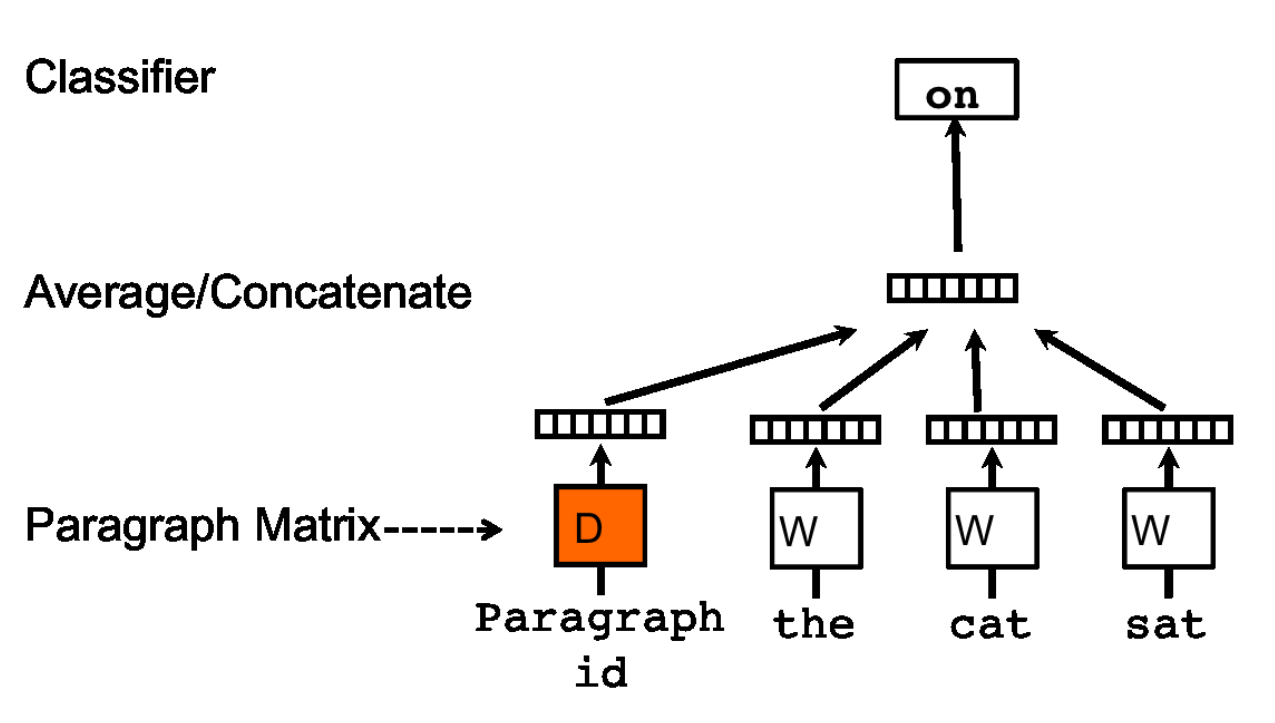
\includegraphics[width=250px]{../chapters/implementation/pics/doc2vec}
	\caption{\label{pic:doc2vec} Visualization of a training step of a Doc2Vec network {\cite{wuWordMoverEmbedding2018}}}
\end{figure}

\subsection{Selection of a document embedding technique}

Summarizing the previously discussed methods by three of their main characteristics - number of hyperparameters, maximum processable document length and type of model - \autoref{tab:overview_doc_embedding}
\begin{table}
	\centering
	\begin{tabular}{ c | c | c | c }
		\hline 
		Technique & Parameters & Max. document length & Type \\ \hline
		Tf-Idf BOW & 0 & unlimited & Probabilistic \\ \hline
		Latent Dirichlet Allocation & 1 & unlimited & Probabilistic \\ \hline
		Doc2Vec & 8 & unlimited & NN \\ \hline
		Word mover's embedding & 1 & unlimited & Kernel method \\ \hline
		BERT & 8 & 512 characters & NN \\ \hline
	\end{tabular}
	\caption{\label{tab:overview_doc_embedding} Table summarizing the key features of different document embedding techniques}
\end{table}


\subsection{Explainability technique: Top words}

\section{Topic extraction}

\subsection{Quality of topic extraction}

\section{Clustering}

\subsection{Explainability technique: Cluster topography }

\section{Reduction into 2D}

\subsection{Explainability technique: Linearization}